%https://www.overleaf.com/learn/latex/Beamer_Presentations:_A_Tutorial_for_Beginners_(Part_2)—Lists,_Columns,_Pictures,_Descriptions_and_Tables

%Usate il link sopra è una guida con tutti i comandi per le slidesss
\documentclass{beamer}

\usepackage{graphicx}           	% Allows including images
\usepackage{booktabs}         	  	% Allows the use of \toprule,
                                					% \midrule and \bottomrule in tables
\usepackage{tikz}               		% add background image

\usepackage{setspace}				%different line spacing can be achieved.
\usepackage{wrapfig}




\title{Laboratorio di Applicazioni Mobili}
\subtitle{Pregetto 2019/2020 - Personal Health Monitor}
\author{
  Matteo Celani
  \texttt{Matricola 0000804303}
 }
\institute{Università di Bologna}
\date{}

\setbeamertemplate{frametitle}[default][center]


\begin{document}

\begin{frame}
\titlepage
\vspace{-1.1cm}
\begin{figure}[htp]

\centering
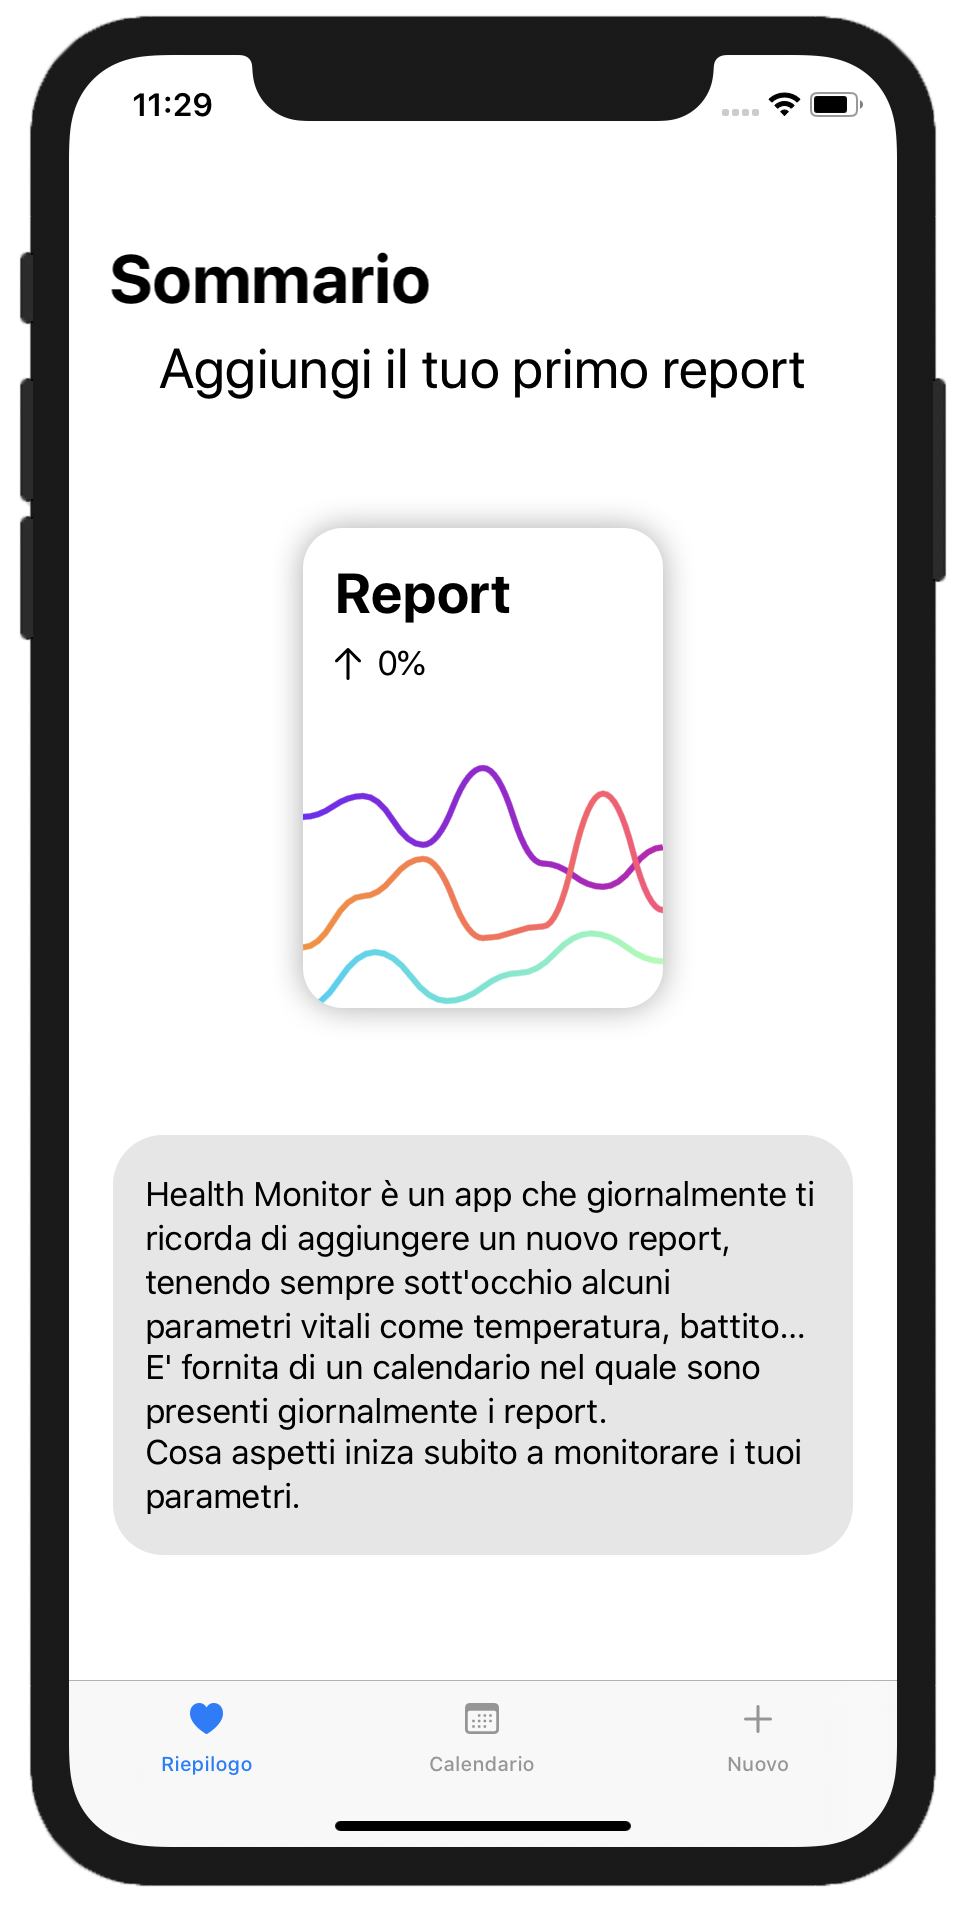
\includegraphics[width=.23\textwidth]{../img/riepilogo_iniziale.png}\hfill
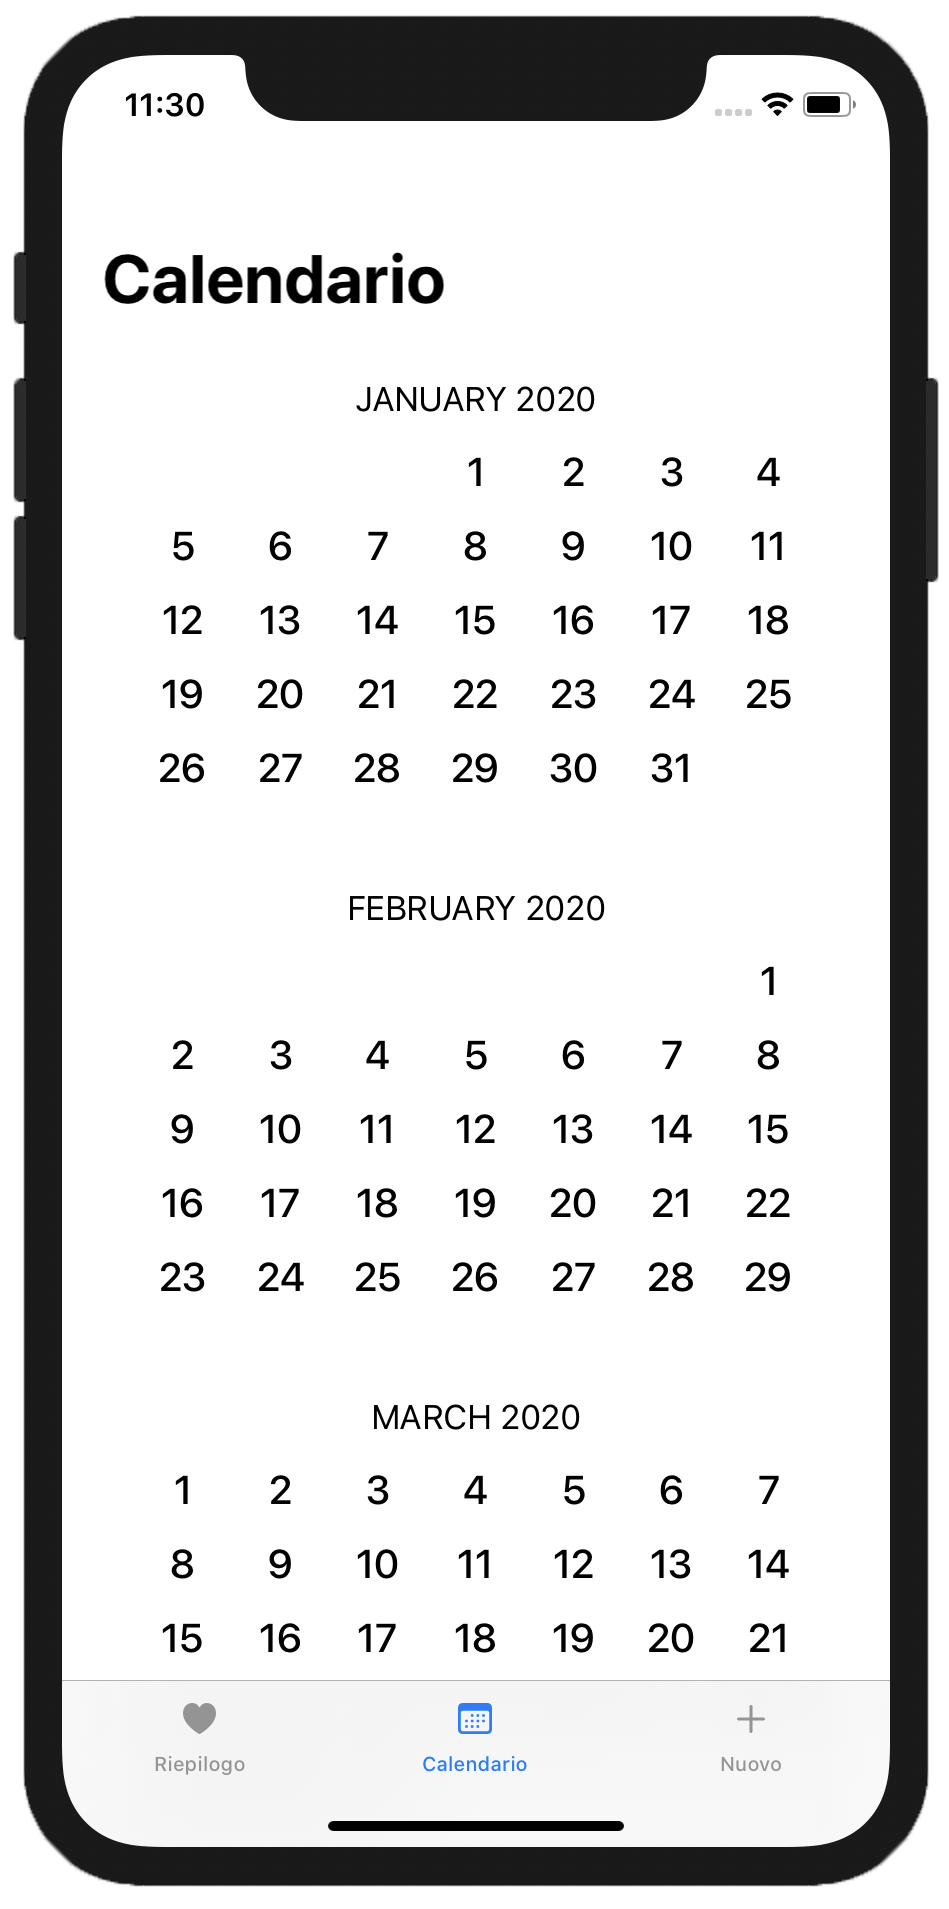
\includegraphics[width=.23\textwidth]{../img/calendario_iniziale.png}\hfill
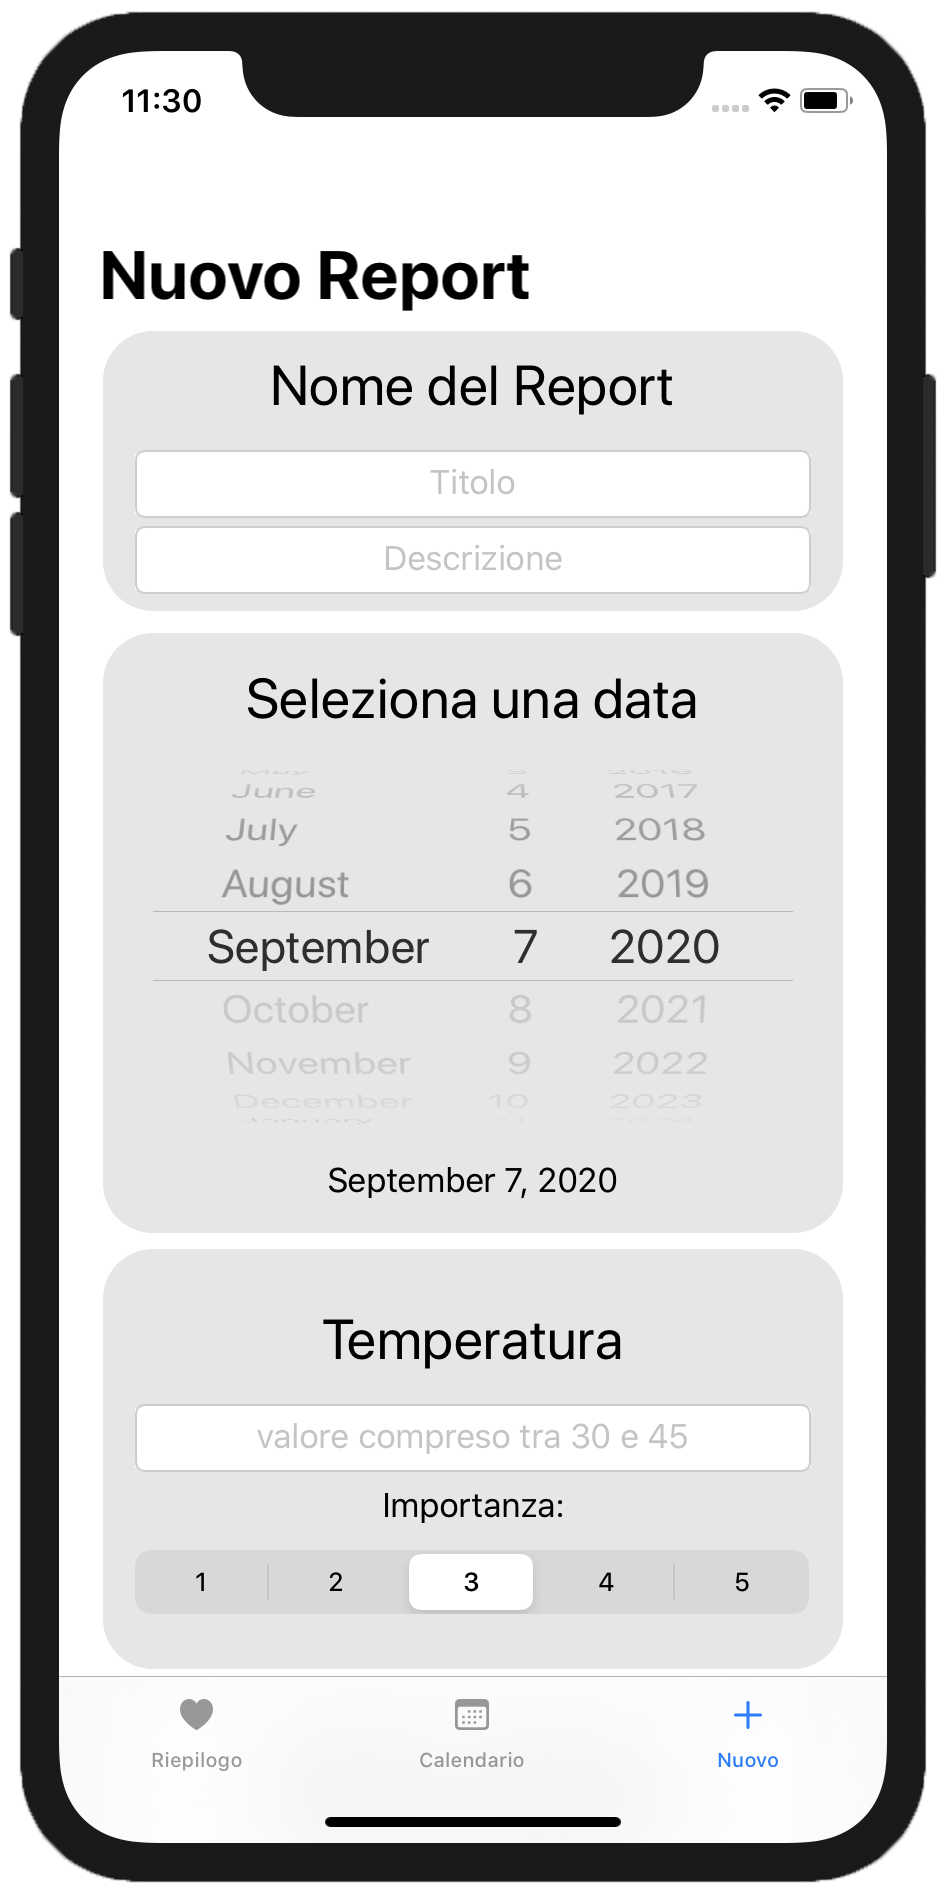
\includegraphics[width=.23\textwidth]{../img/nuovo_iniziale.png}

\end{figure}
\end{frame}

\begin{frame}
\frametitle{Specifiche}
\framesubtitle{Health Monitor}	   
\begin{columns}
\column{0.5\textwidth}
Health Monitor è un'app per caricare e monitorare alcuni parametri vitali. L'utente può:
\begin{itemize}
  \item caricare nuovi report;
  \item visualizzare i report in un calendario organizzato o tramite grafici;
  \item modificare report presenti;
  \item eliminare report.
\end{itemize}
	
\column{0.5\textwidth}
	\centering 
	\begin{figure}[h]
	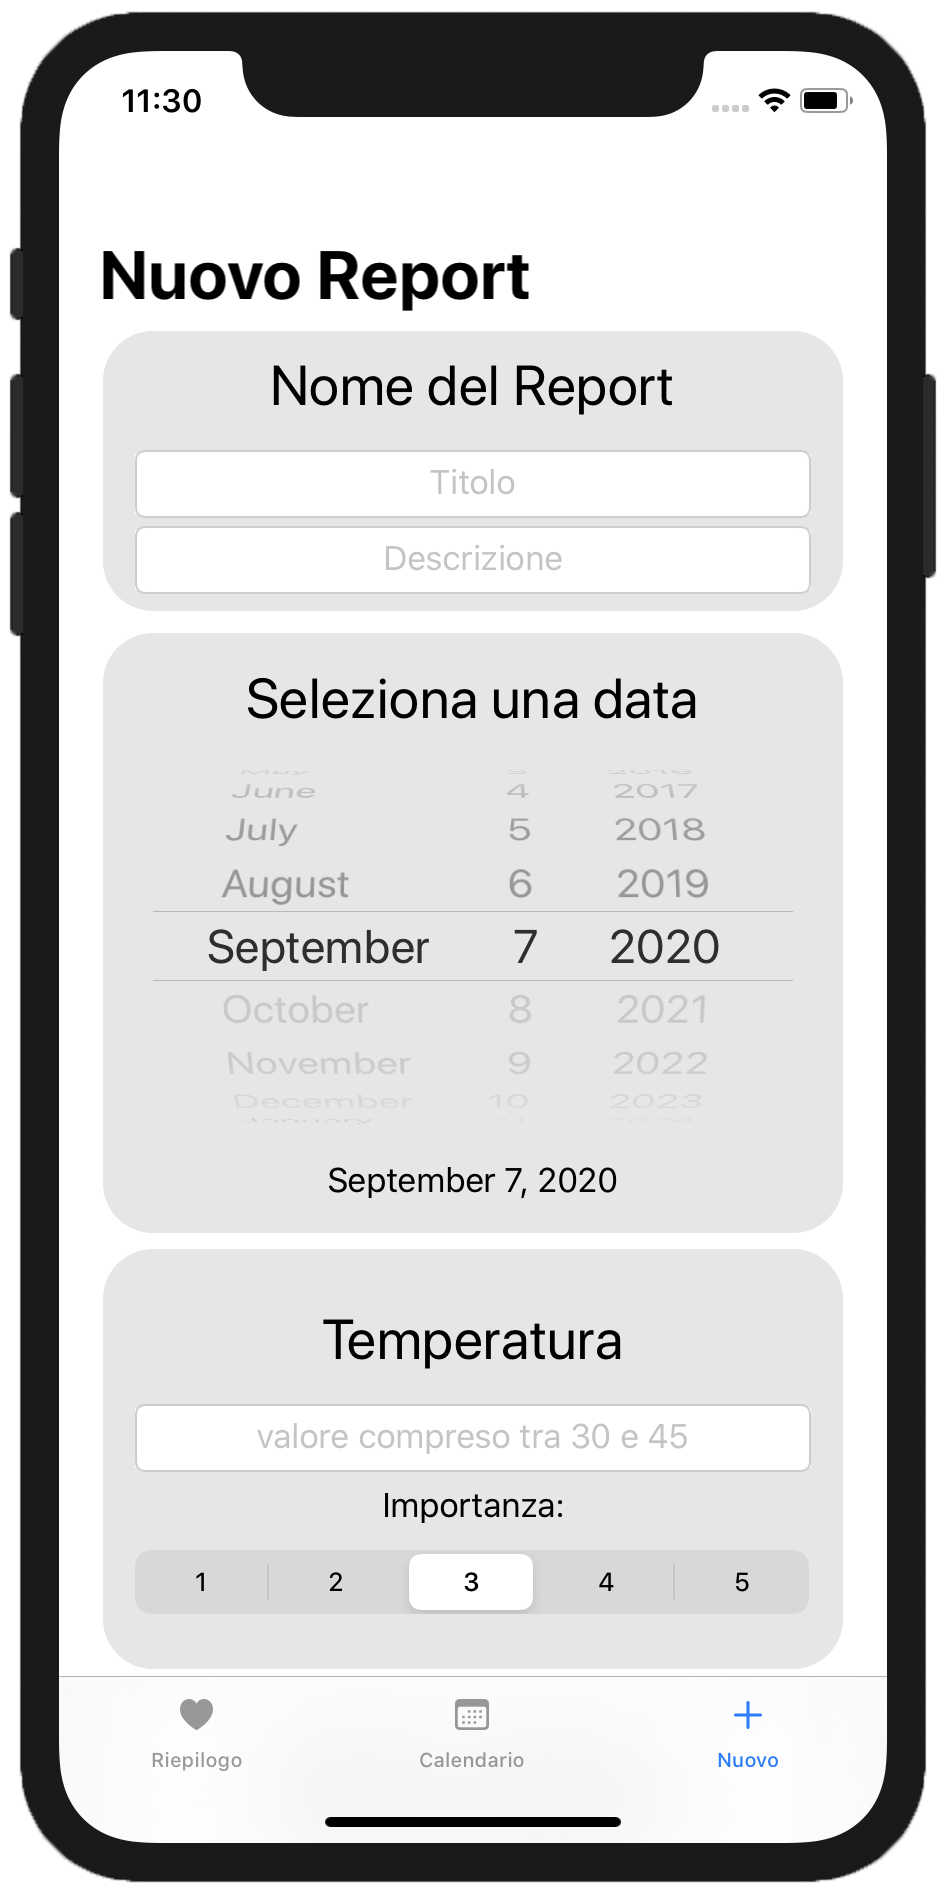
\includegraphics[width=0.55\textwidth]{../img/nuovo_iniziale.png}
	\caption{Nuovo report}
	\end{figure}
\end{columns}
\end{frame}

\begin{frame}
\frametitle{Specifiche}
\framesubtitle{I Report}	   
\begin{columns}
\column{0.5\textwidth}
	\centering 
	\begin{figure}[h]
	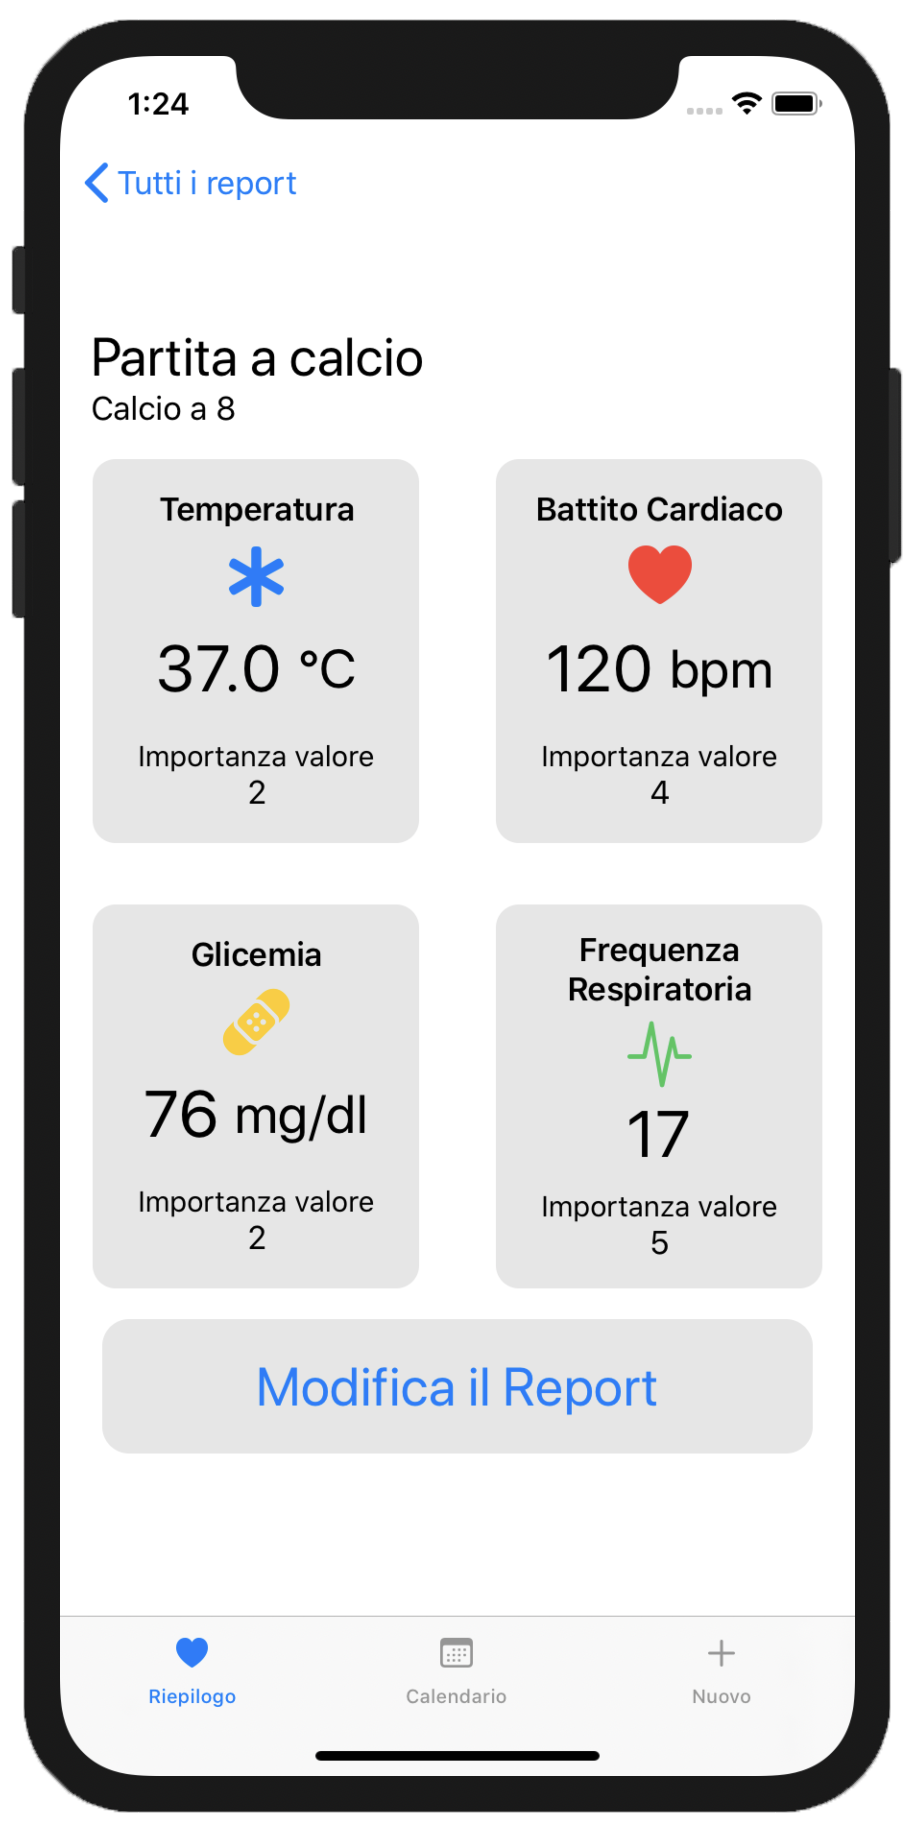
\includegraphics[width=0.55\textwidth]{../img/ReportView1.png}
	\caption{Dettagli Report}
	\end{figure}
	
\column{0.5\textwidth}
I report vengono salvati e mantenuti in memoria attraverso i Core Data. Essi sono composti da 4 valori e ogni valore ha un’importanza che va da 1 a 5.\\
\vspace{0.3cm}
\begin{itemize}
  \item temperatura;
  \item battito cardiaco;
  \item glicemia;
  \item frequenza respiratoria.
\end{itemize}
\end{columns}
\end{frame}

\begin{frame}
\frametitle{Tecnologie e strumenti utilizzati}
\begin{columns}
\column{0.5\textwidth}
Tecnologie:
	\begin{itemize}
 	 \item Swift 5 
  	\item SwiftUI
  	\item Core Data
	\end{itemize}
	
\column{0.5\textwidth}
Strumenti
\begin{itemize}
  \item xCode 11
  \item iPhone 11
  \item Simulatore iOS
\end{itemize}
\end{columns}
	\vspace{0.4cm}
	Requisiti minimi: iOS 13.0+ , Xcode 11+ , Swift 5.1+ \\
		\vspace{0.4cm}
      \centering  \begin{tabular}{c}
        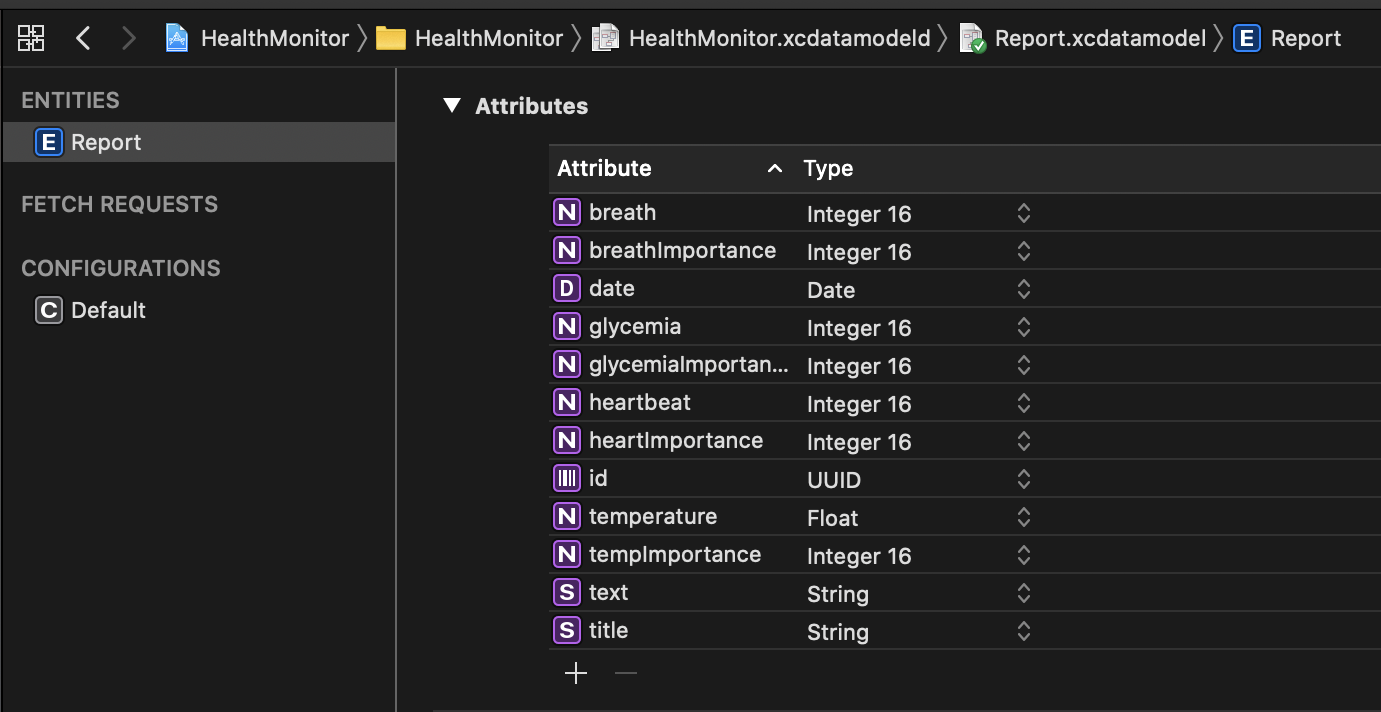
\includegraphics[width=8cm]{../img/CoreData.png}
      \end{tabular}
\end{frame}

\begin{frame}
\frametitle{NavigationView}
  \begin{figure}[h]
  	\centering 
        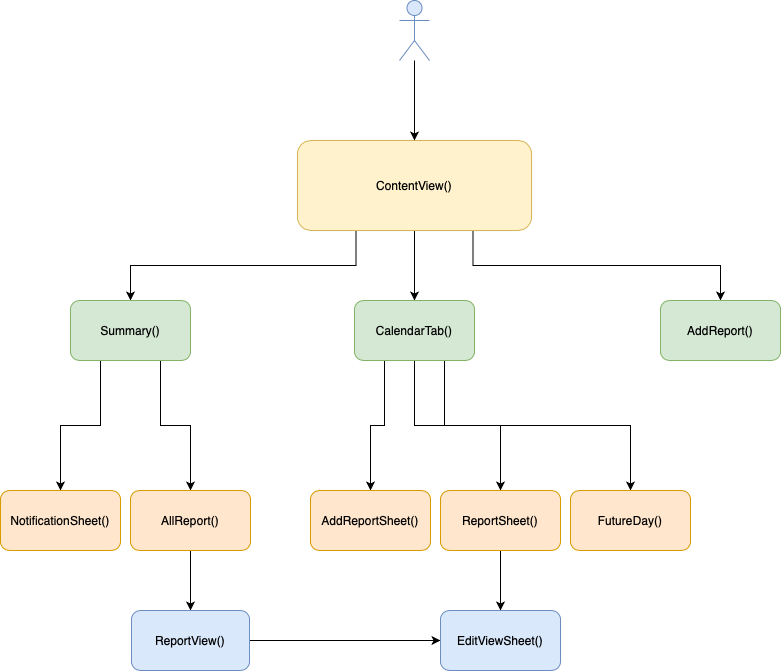
\includegraphics[width=9cm]{../img/NavigationView.png}
   \end{figure}
\end{frame}

\begin{frame}
\frametitle{Aggiungi un Report}
\begin{columns}
\column{0.5\textwidth}
In HealthMonitor vogliamo aggiungere nuovi report quindi questa operazione è stata semplificata il più possibile con una tab specifica.
\column{0.5\textwidth}
  \centering  
  \begin{figure}[h]
        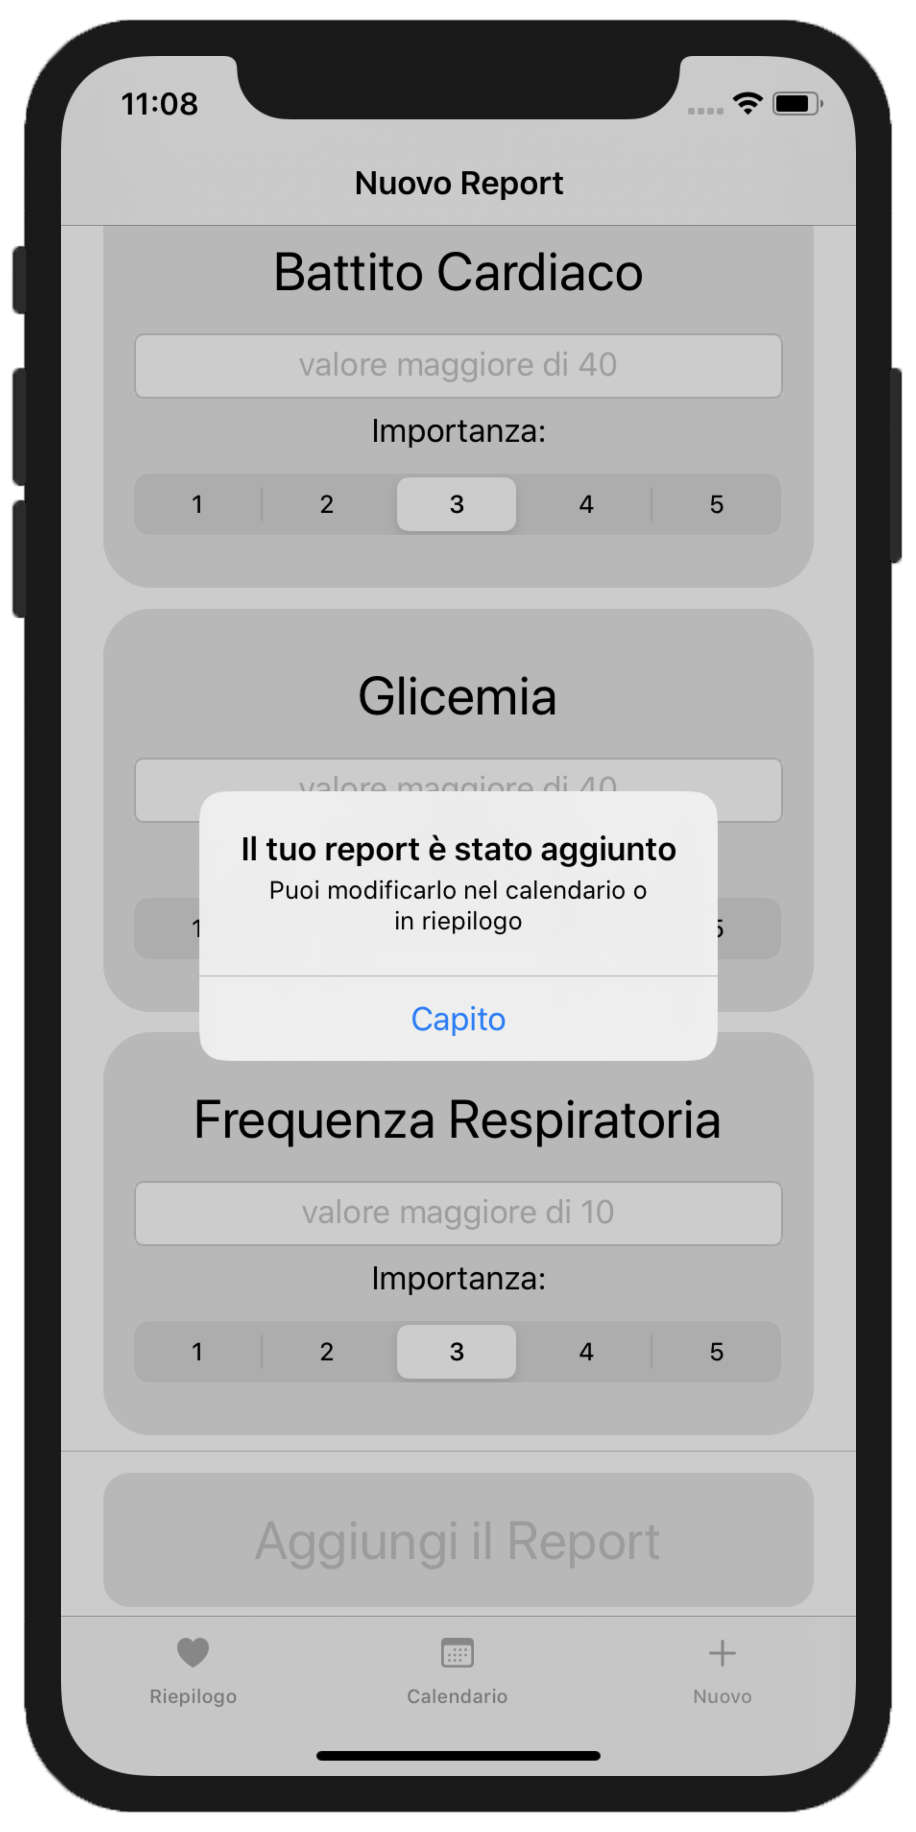
\includegraphics[width=0.55\textwidth]{../img/nuovo2.png}
        \caption{Report Aggiunto}
   \end{figure}
\end{columns}
\end{frame}

\begin{frame}
\frametitle{Calendario}
\begin{columns}
\column{0.5\textwidth}
	\begin{figure}[h]
        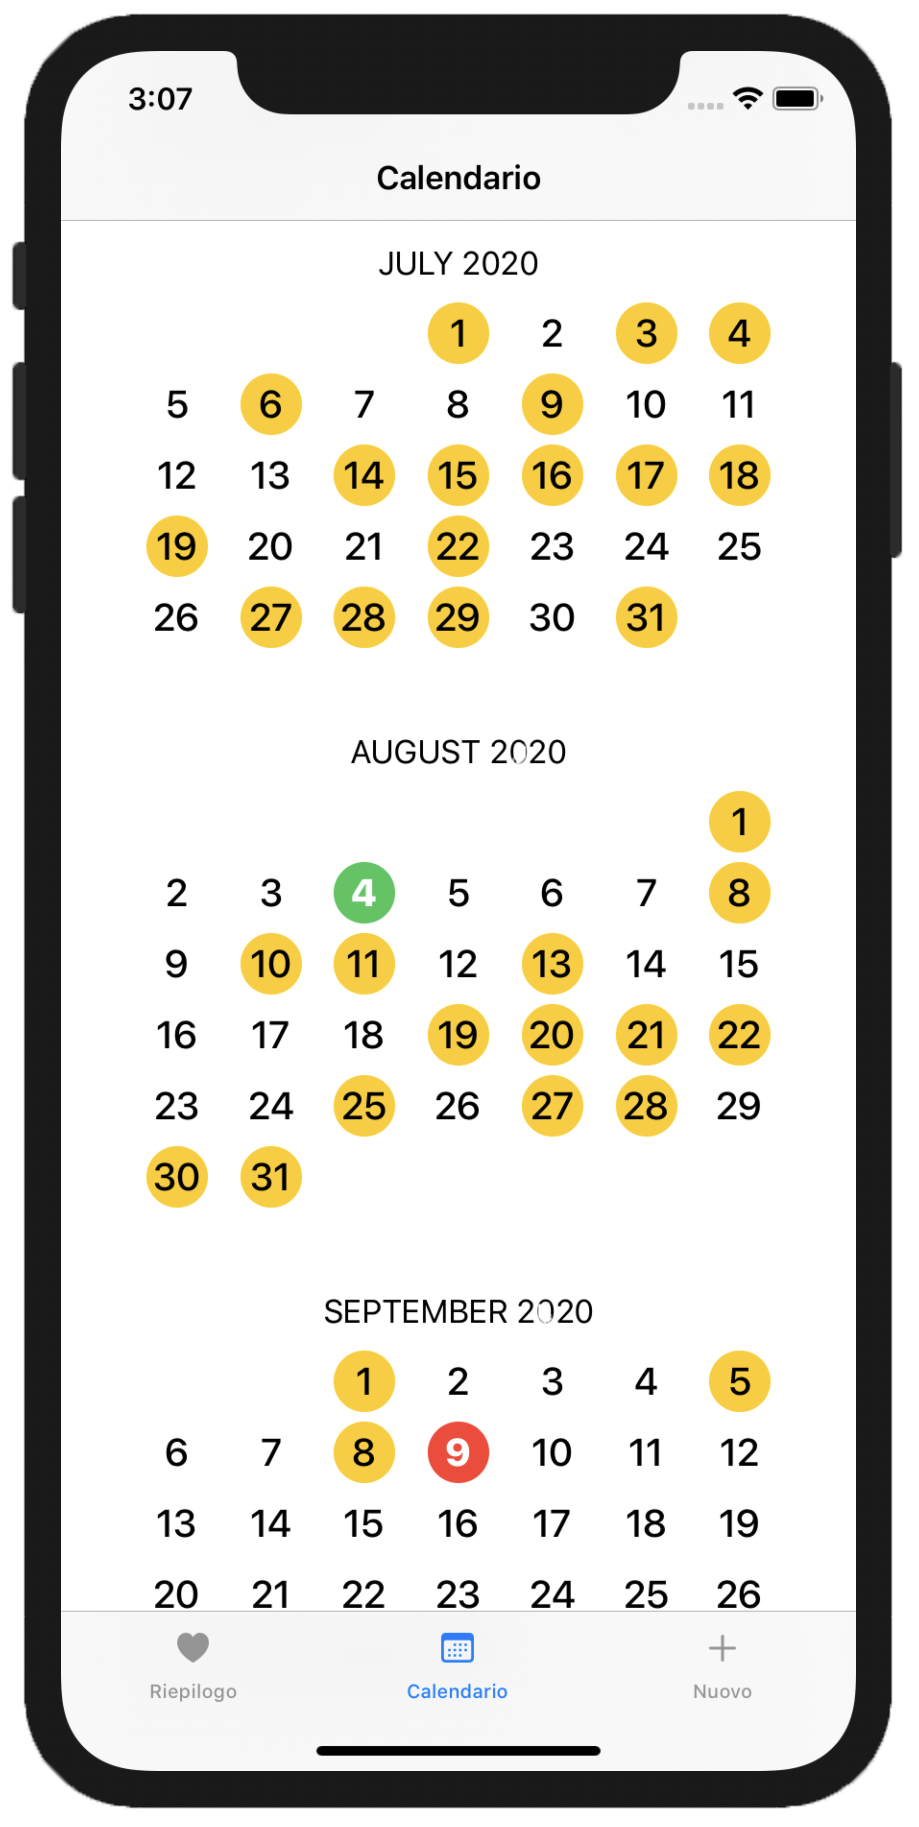
\includegraphics[width=0.55\textwidth]{../img/calendario1.png}
        \caption{Calendario con Report}
   \end{figure}
   
\column{0.5\textwidth}
  \begin{itemize}
	\item Creare report per uno specifico giorno
	\item Visualizzare giorni con report presenti e non presenti
	\item Visualizzare i dettagli di un report
	\item Modificare un report per uno specifico giorno
	\item Eliminare report per uno specifico giorno
  \end{itemize}
\end{columns}
\end{frame}

\begin{frame}
\frametitle {Sommario}
\begin{columns}
\column{0.5\textwidth}
  \begin{itemize}
	\item Visualizzare grafici con valori ordinati per data 
	\item Visualizzare tutti i report
  \end{itemize}
\column{0.5\textwidth}
	\begin{figure}[h]
        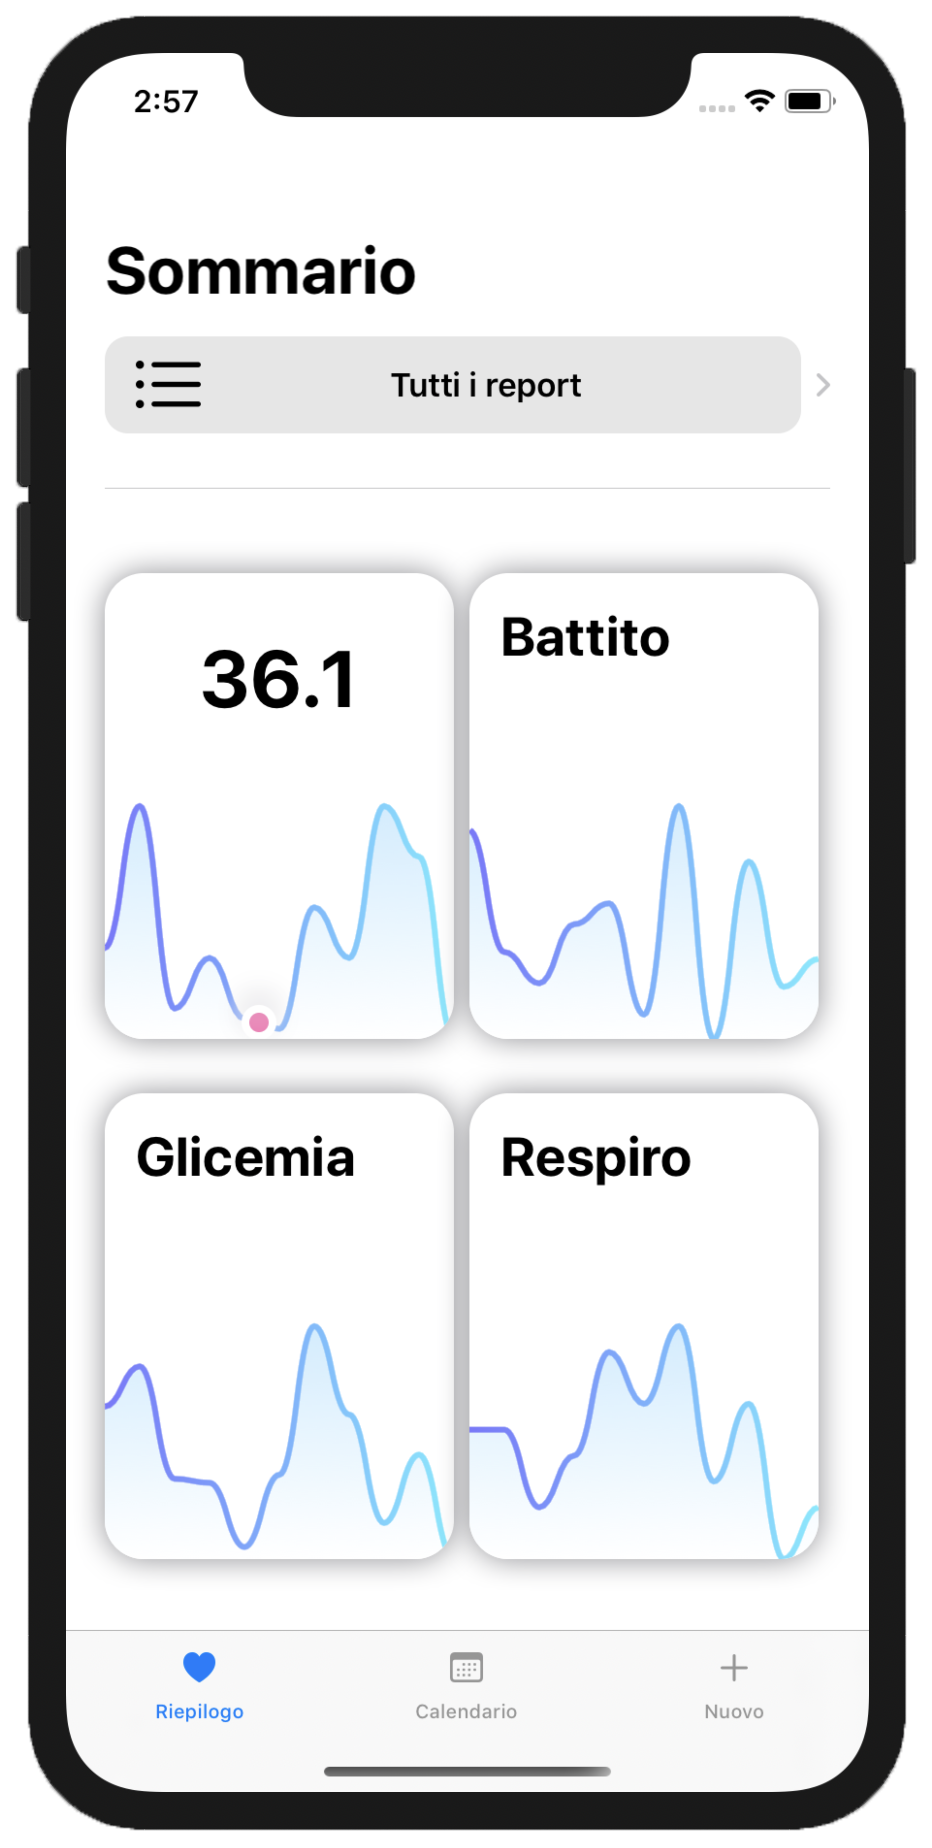
\includegraphics[width=0.55\textwidth]{../img/grafico2.png}
        \caption{Sommario con dati}
   \end{figure}
\end{columns}
\end{frame}

\begin{frame}
\frametitle{Sommario}
\framesubtitle{Tutti i report}
\begin{columns}
\column{0.5\textwidth}
	\begin{figure}[h]
        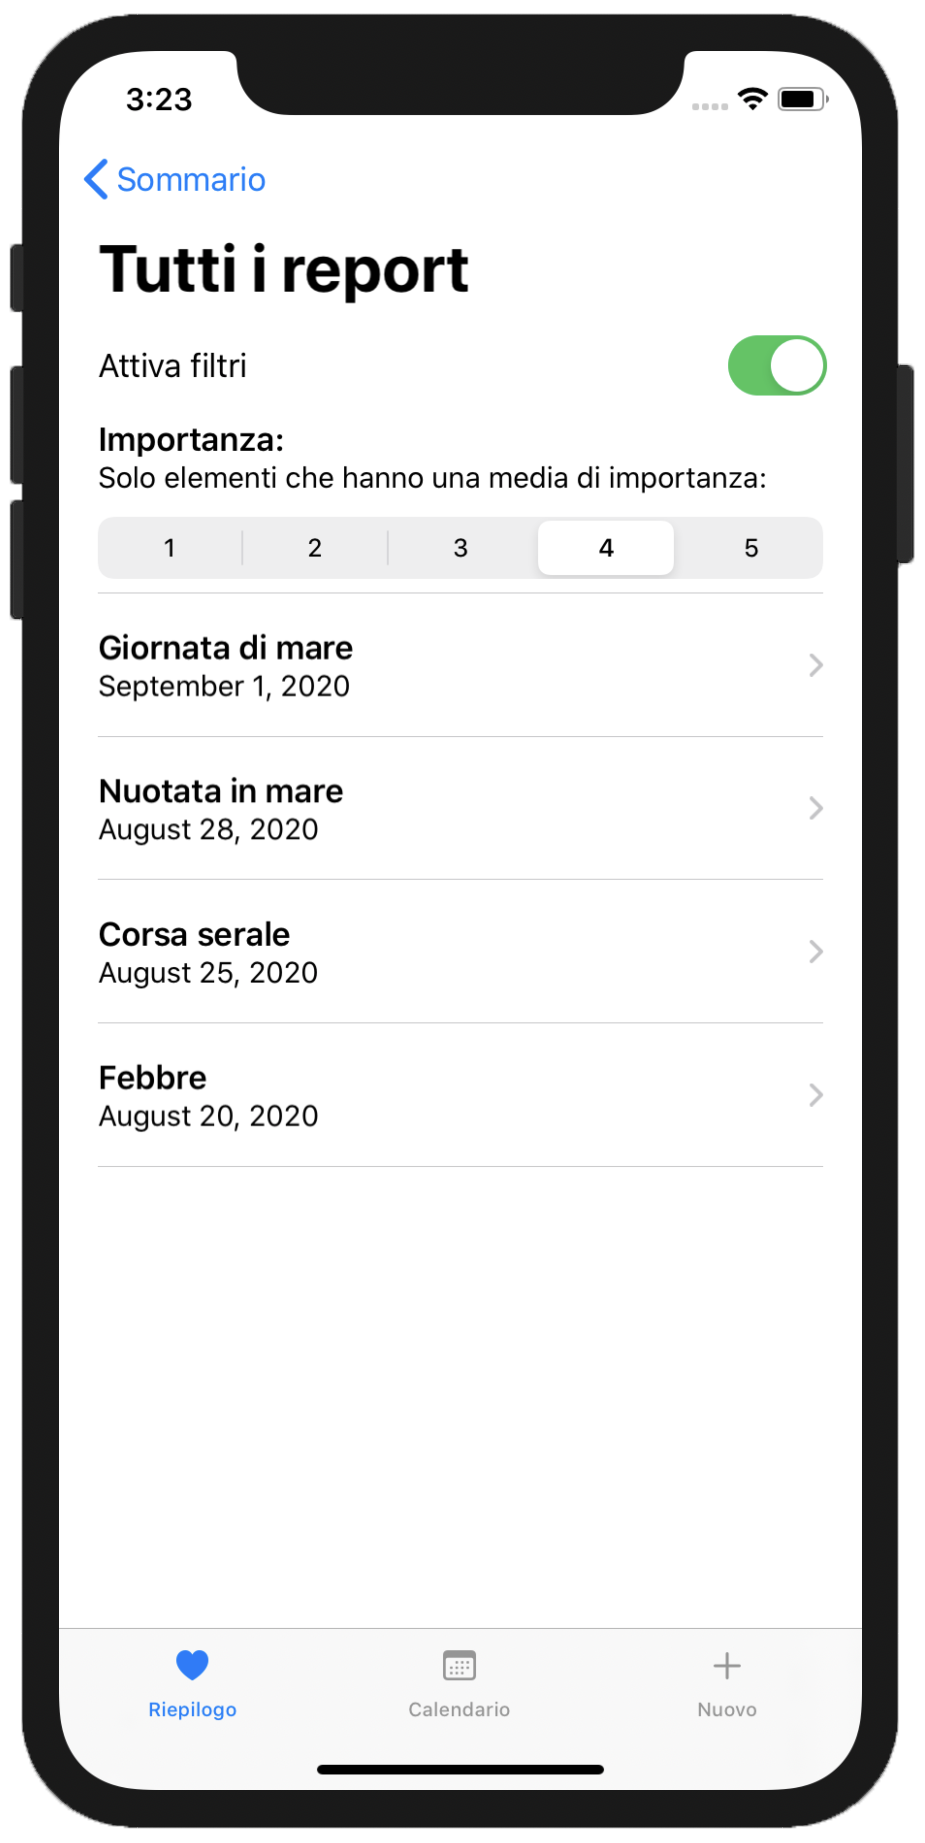
\includegraphics[width=0.55\textwidth]{../img/tutti3.png}
        \caption{Report con filtri}
   \end{figure}
   
\column{0.5\textwidth}
  \begin{itemize}
	\item Visualizzare una lista completa di report organizzati per data
	\item Visualizzare i report attraverso filtri
	\item Visualizzare i dettagli del report
	\item Modificare un report
	\item Eliminare report
  \end{itemize}
\end{columns}
\end{frame}

\begin{frame}
\frametitle{Sommario}
\framesubtitle{Notifiche}
\begin{columns}
\column{0.5\textwidth}
  \begin{itemize}
	\item Attivare le notifiche
	\item Settare un orario per le notifiche
	\item Accedere all'app tramite le notifiche
  \end{itemize}
\column{0.5\textwidth}
	\begin{figure}[h]
	\centering
        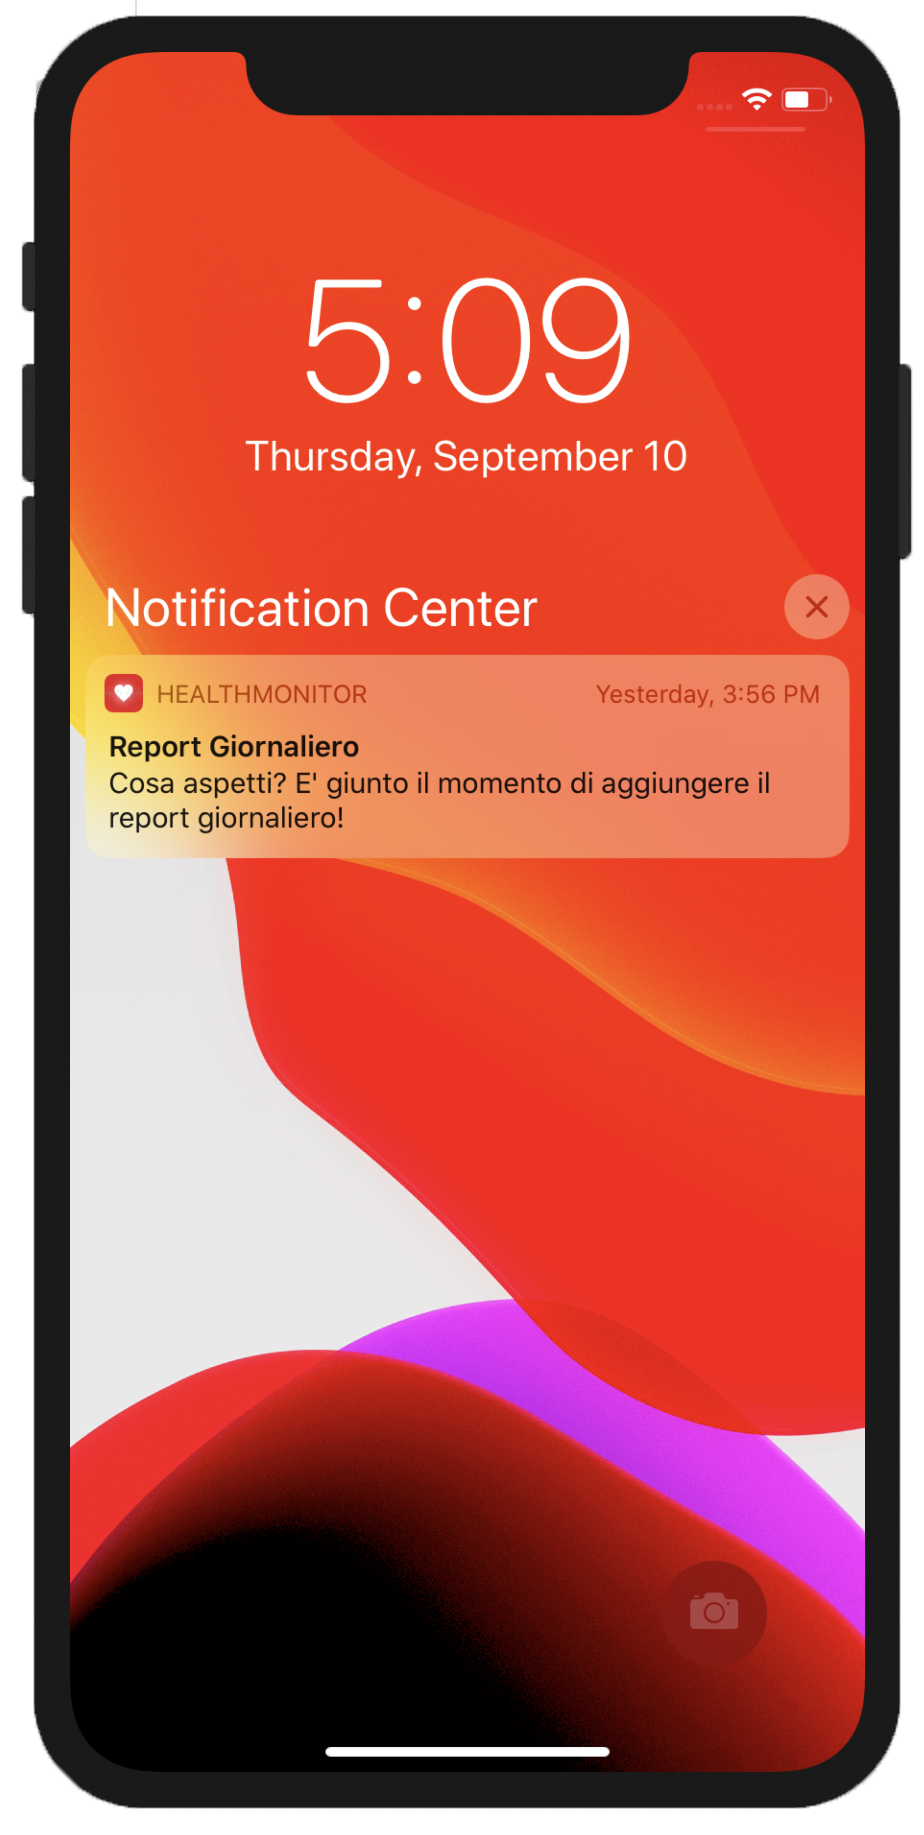
\includegraphics[width=0.55\textwidth]{../img/notifiche3.png}
        \caption{Notifica Giornaliera}
   \end{figure}
\end{columns}
\end{frame}

\begin{frame}
\frametitle{Health Monitor}
\framesubtitle{Impressioni Finali}
  \begin{itemize}
  	\item Swift ha una pessima gestione delle tastiere
	\item SwiftUI più ordinato, intuitivo e di facile utilizzo rispetto Storyboard
  \end{itemize}
\begin{figure}[htp]

\centering
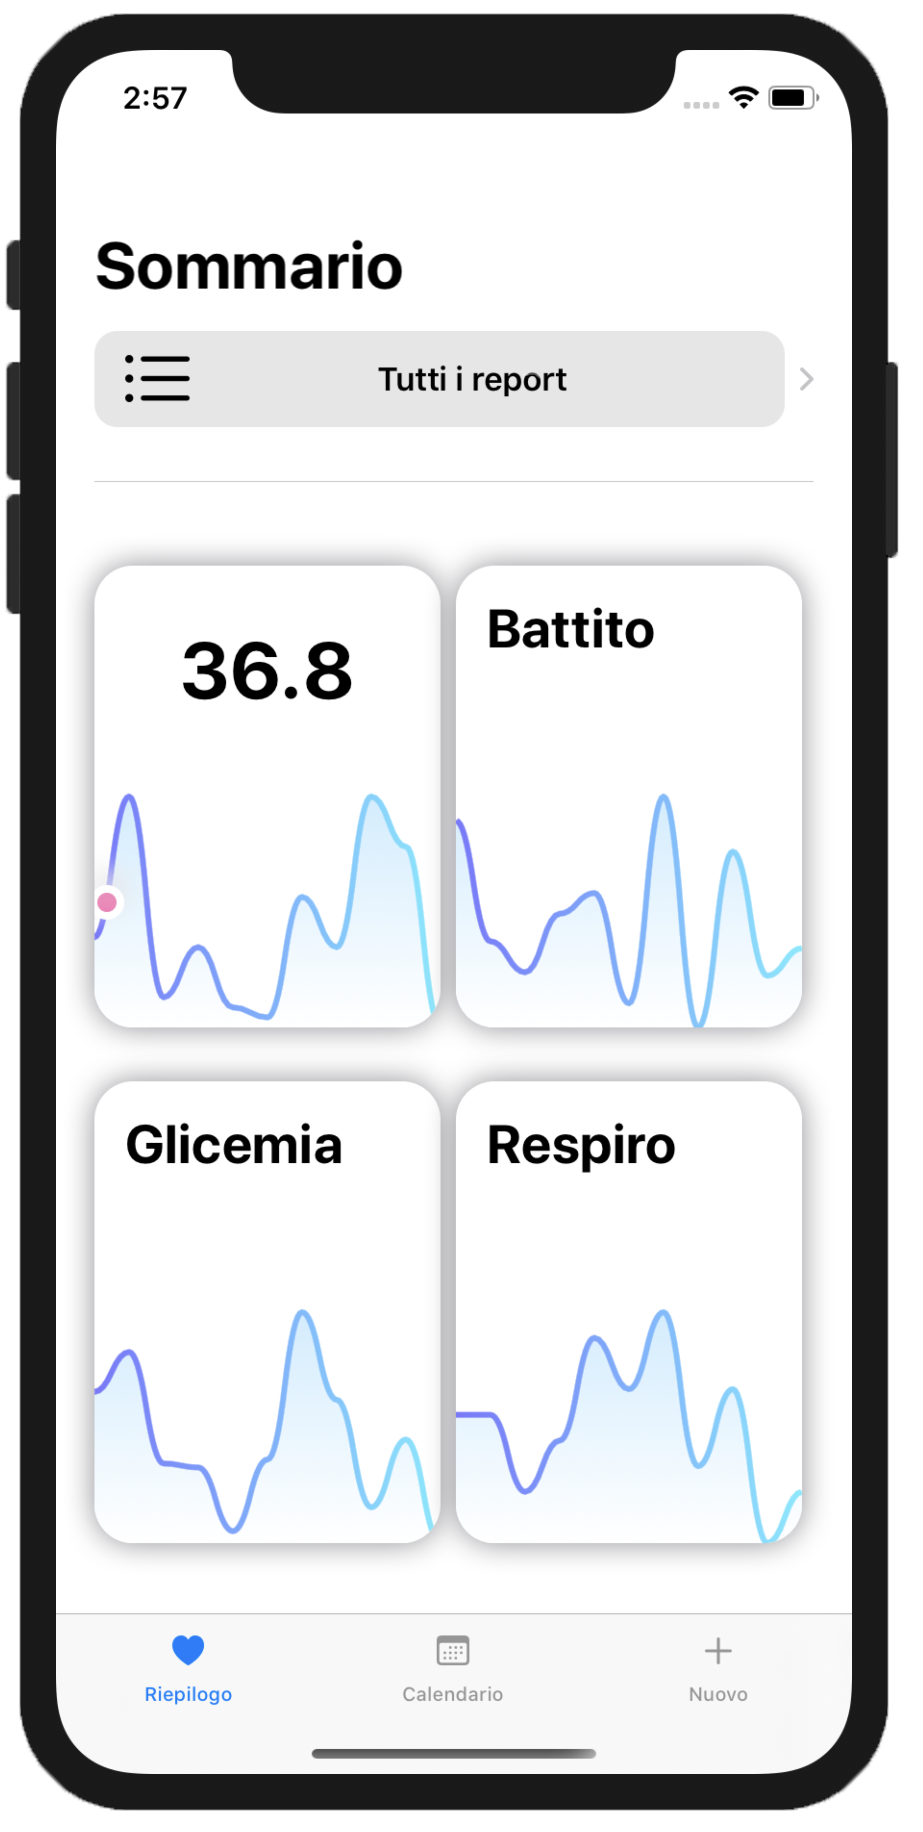
\includegraphics[width=.25\textwidth]{../img/grafico1.png}\hfill
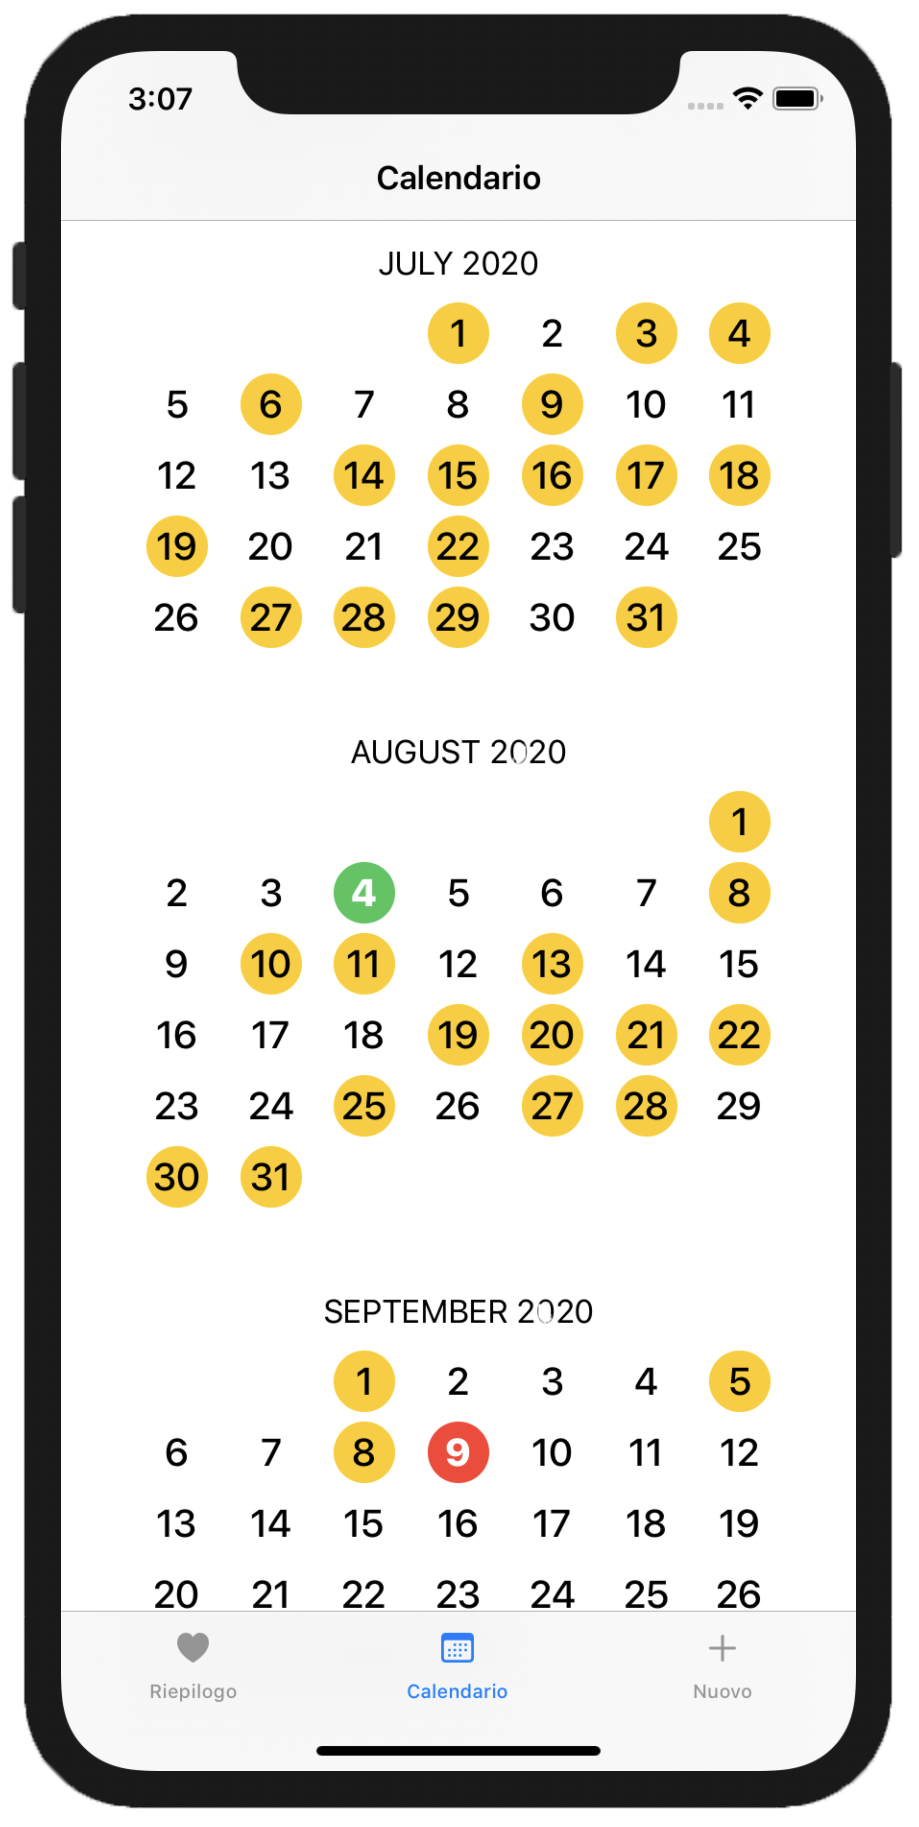
\includegraphics[width=.25\textwidth]{../img/calendario1.png}\hfill
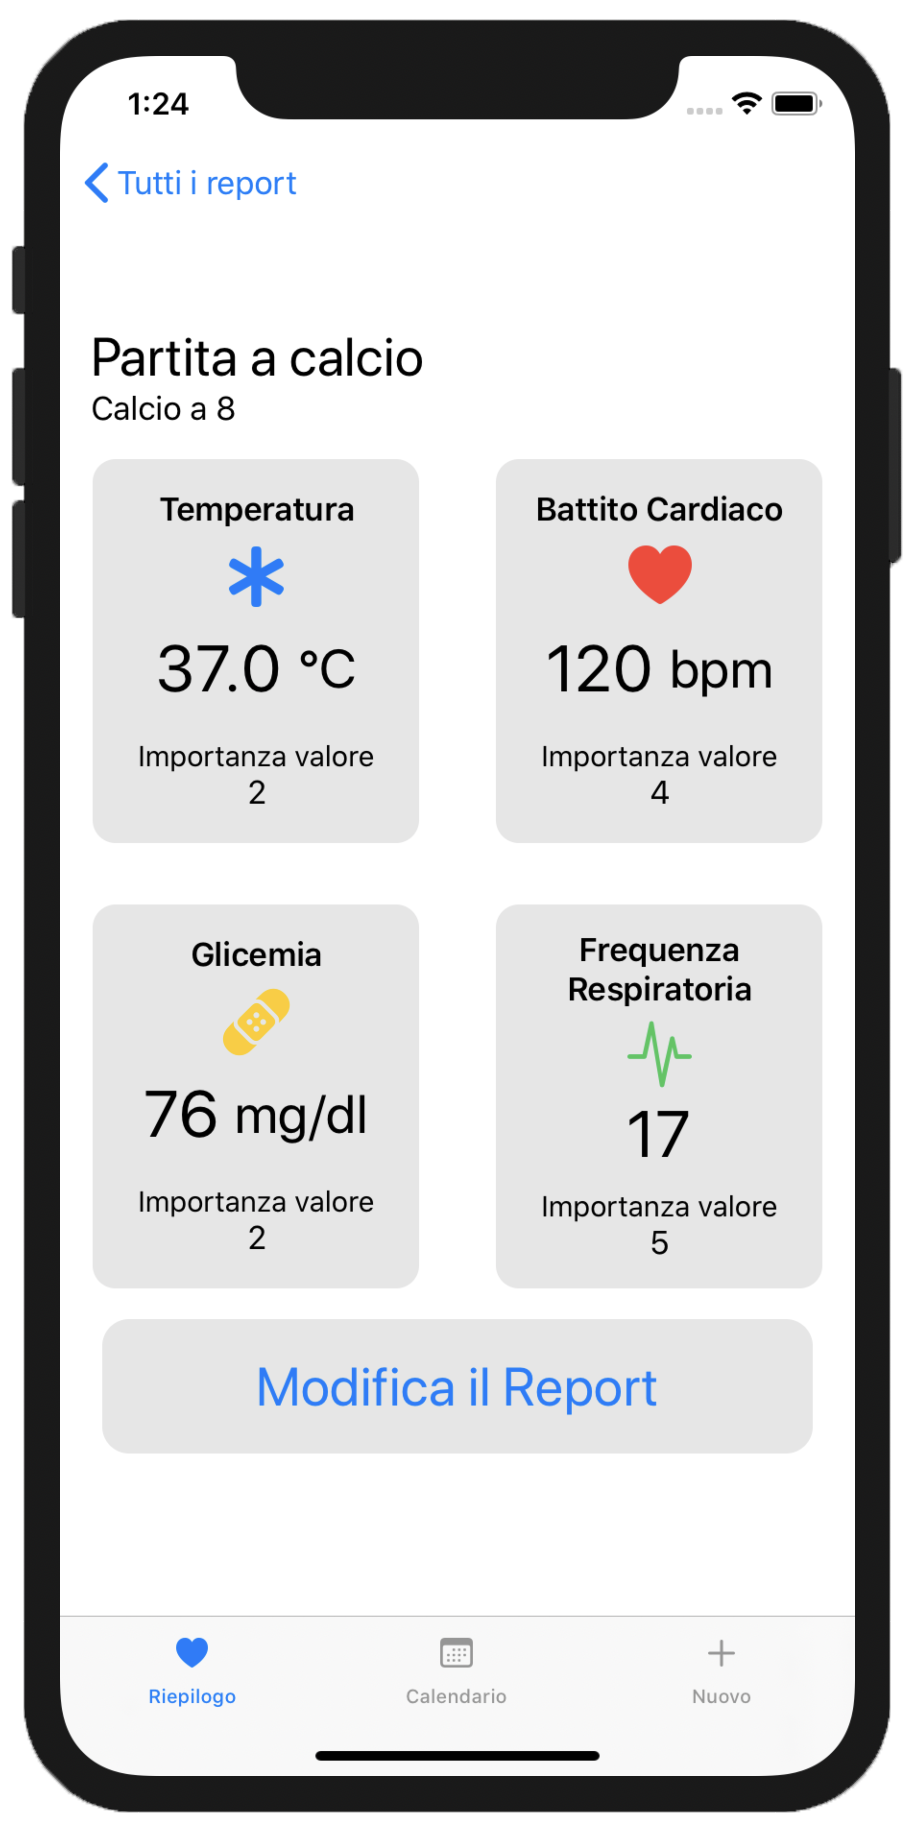
\includegraphics[width=.25\textwidth]{../img/ReportView1.png}

\end{figure}

\end{frame}

\end{document}
